\chapter{Résultats de simulation et analyse du modèle à état discret (\textit{2 pages max})}
\label{ch:simu}

Afin de valider les constats émis au chapitre \ref{ch:modele_discret}, cette partie se propose d'effectuer des simulations numériques afin d'étudier la stabilité des différents points d'équilibre.

Pour ce faire, ce chapitre se consacre à l'analyse de bifurcation, comme déjà utilisée dans \cite{ChaosControl}. Le code fourni en complément du rapport est fortement basé sur le tutoriel d'analyse de bifurcation pour Python présenté en \cite{bifurc} avec l'exemple de l'équation logistique.

Afin d'obtenir un diagramme de bifurcation, il a fallu décider d'un paramètre pertinent à faire varier et choisir les valeurs auxquelles fixer tous les autres paramètres. En repartant de l'équation logistique présentée dans \cite{bifurc}, nous avons décidé de faire varier le paramètre $\alpha$, mais aussi d'imposer les deux conditions suivantes : $\gamma = \alpha$ comme dans l'équation logistique et $\beta = 0.1 \alpha$ afin de faire un lien entre la facilité de la chasse et le nombre de prédateurs.

\begin{figure}
    \begin{center}
		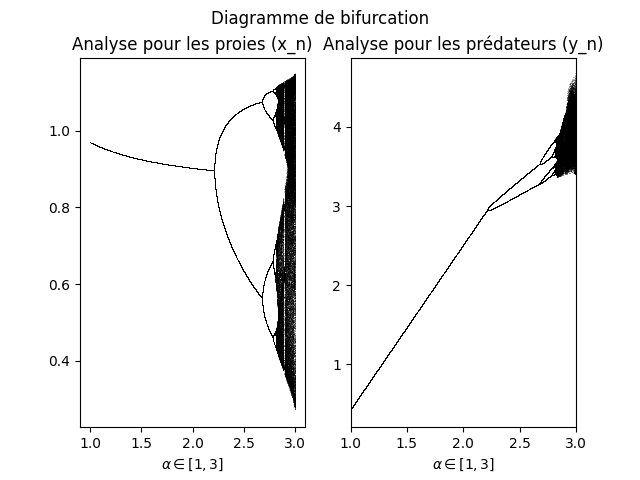
\includegraphics[width=17cm]{figures/Bifurcation_1.png}
	\end{center}
	\caption{Analyse de bifurcation pour les paramètres $\alpha \in [1, 3]$; $\beta = 0.08$; $\gamma = \alpha$; $\rho = 0.08$; $\sigma = 0.1*\alpha$ et $\nu = 0.04$ avec les conditions initiales $x_0 = 1.1$ et $y_0 = 1$}
    \label{fig:bifurc}
\end{figure}

Afin d'analyser les résultats obtenus à la figure \ref{fig:bifurc}, on peut comparer les conditions de stabilité mises en lumière sur le diagramme de bifurcation avec les conditions de stabilités sur les valeurs propres du linéarisé tangent à l'équilibre $(x^*, y^*)$, comme décrit en (\ref{eq:matrices equilibre}).

Par lecturre graphique, on trouve que la valeur limite de bifurcation est $\alpha = 2.2$. Vérifions par le calcul la pertinence de cette valeur par rapport au modèle théorique.

Après calcul, on obtient tout d'abord comme valeurs pour $x^*$ et $y^*$ les valeurs suivantes : $x^* = 0.894$ et $y^* = 2.904$, ce qui est cohérent avec ce que l'on observe sur le diagramme de bifurcation aux alentours de $\alpha = 2.2$.



Le Chapitre \ref{ch:simu} porte sur la \textit{présentation des résultats de simulation} (ne pas oublier de préciser les valeurs numériques des paramètres considérés) et l’\textit{analyse des résultats de simulation obtenus en utilisant le modèle à état discret}.
Ce chapitre permettra de valider en simulation le modèle à état continu, complétant les réponses aux questions I.1, I.2 et I.3 du sujet.
